\section{Our Approach}

\subsection{Pig Latin Features}
\begin{frame}{Features}
\begin{itemize}
	\item DataFlow Language: 
	\begin{itemize}
		\item Programmer defines a sequence of statements where each carries out a single 					  data transformation. The output relation of each statement is stored in an  					  identifier to be used later in the program.
	\end{itemize}
	\item User Defined Functions:
	\begin{itemize}
		\item User defined functions provide the flexibility to perform specialized data 				 	  processing tasks.
	\end{itemize}
	\item Abstract Parallelism:
	\begin{itemize}
		\item Pig Latin programs are represented a sequential way to define the query 					      statements abstracting away the underlying parallelism performed through the 					  map-reduce tasks.
	\end{itemize}
\end{itemize}
\end{frame}

\subsection{Formalism}
\begin{frame}{Four Stages of Pig Programs}
\begin{itemize}
	\item A Pig Latin program passes through four stages of compilation:
	\begin{itemize}
		\item Pig Latin Program
		\item Logical Plan
		\item Physical Plan
		\item Map Reduce Phase
	\end{itemize}
	\item The logical plan is an one-to-one mapping from Pig Latin Program and the in Map-				  Reduces phase is executed by assigning physical operators to corresponding map-				  reduce jobs. So we've started our formalism by defining the calculus for Logical 				  plan and Map-Reduce in terms of Pig Latin programs.
\end{itemize}
\end{frame}

\subsection{Formalism for Logical Plan}
\begin{frame}{Types:}
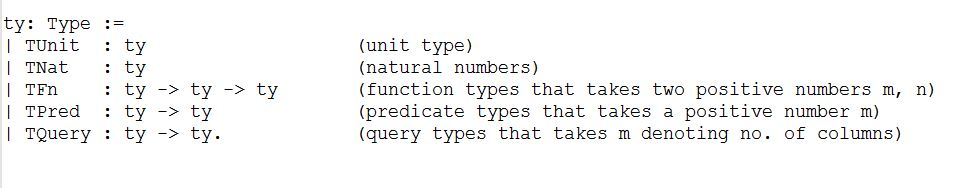
\includegraphics[scale=0.45]{Images/Types.JPG} 
\end{frame}

\begin{frame}{Queries: }
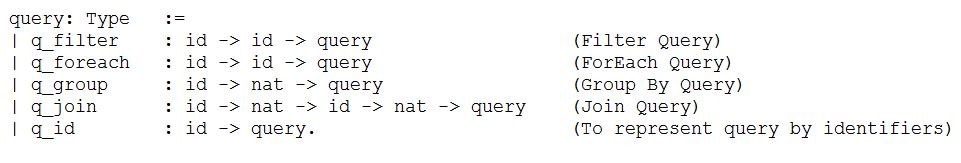
\includegraphics[scale=0.45]{Images/Queries.JPG} 
\end{frame} 

\begin{frame}{Statements: }
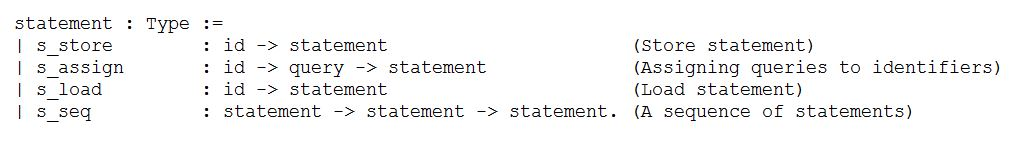
\includegraphics[scale =0.40]{Images/Statements.JPG} 
\end{frame} 

\begin{frame}{Typing Rules for Queries: }
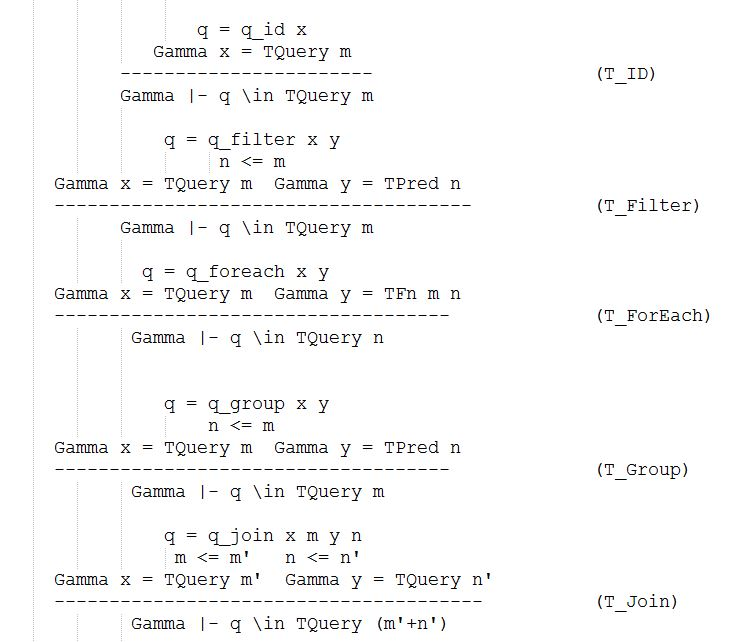
\includegraphics[scale =0.35]{Images/TypingRules_Query.JPG} 
\end{frame} 

\begin{frame}{Typing Rules for Statements: }
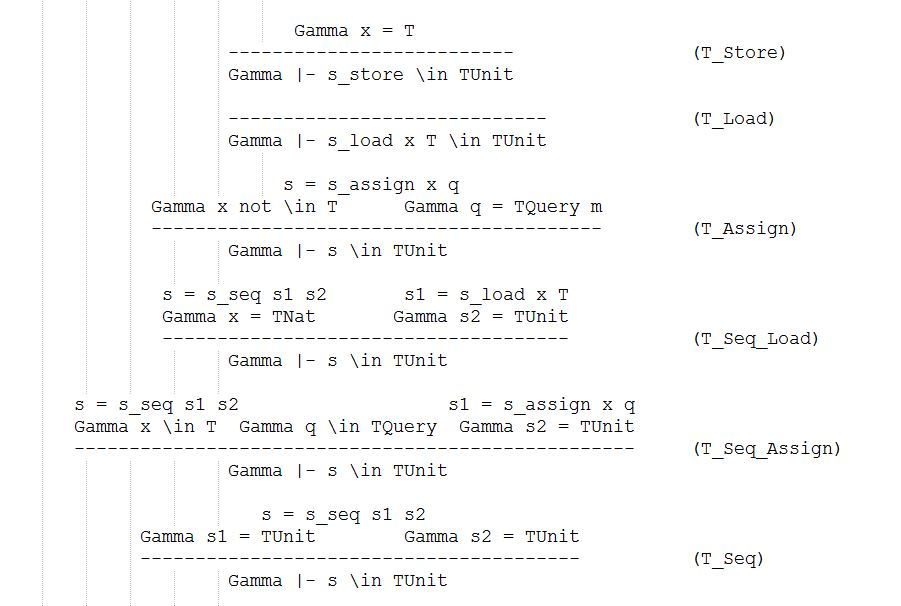
\includegraphics[scale =0.35]{Images/TypingRules_Statements.JPG} 
\end{frame}

%\subsection{Stages}
%\begin{frame}
%\begin{itemize}
%  \frametitle{Stages of Project Development}
%
%  \item Identify program equivalency (correctness) properties:
%  \begin{itemize}
%    \item Initially just functional equivalence?
%  \end{itemize}
%
%  \item Identify Pig programs over which we will write proofs:
%  \begin{itemize}
%    \item Programs with limited data types?
%    \item Programs without user defined functions (UDFs)?
%    \item Programs with some subset of UDFs?
%    \item All well-typed programs?
%  \end{itemize}
%
%  \item Implement all of this in Coq:
%  \begin{itemize}
%    \item Two languages.
%    \item Two semantic models.
%    \item Existing compilation algo.
%    \item Prove correctness/equivalency w.r.t. this compilation algo.
%  \end{itemize}
%
%\end{itemize}
%\end{frame}
%
%\subsection{Operational Semantics}
%\begin{frame}
%  \frametitle{Concurrency in Operational Semantics}
%  We expect that Pig should be able to modeled with sequential or non-concurrent
%  semantics, whereas MapReduce should be modeled with concurrent semantics.
%\end{frame}
%
%\begin{frame}
%  \frametitle{Concern}
%  Our correctness proofs should be performed over all (admissible) concurrent
%  executions and w.r.t. a parameterized number of mappers and reducers.
%\end{frame}
%
%\begin{frame}
%  \frametitle{Nondeterministic MapReduce Operational Semantics}
%  \begin{figure}
%    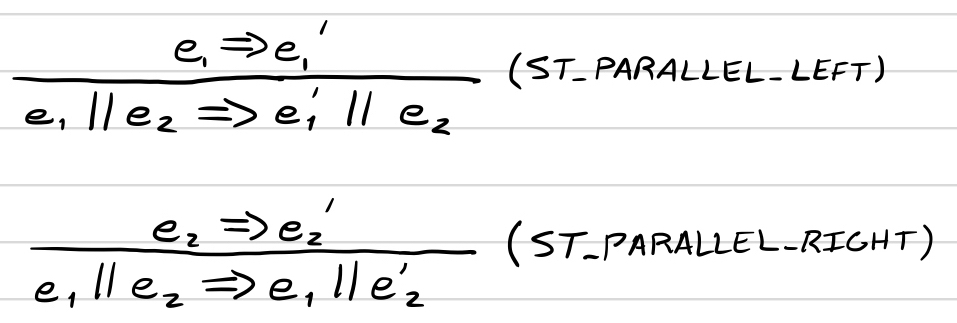
\includegraphics[scale=0.33]{img/ST_PARALLEL.jpeg}
%    \caption{Nondeterminism of two MapReduce reduction rules should enable
%             semantics to model the uncertain ordering by which concurrent tasks
%             are performed.}
%  \end{figure}
%\end{frame}
%
%\begin{frame}
%  \frametitle{Nondeterministic MapReduce Operational Semantics}
%  \begin{figure}
%    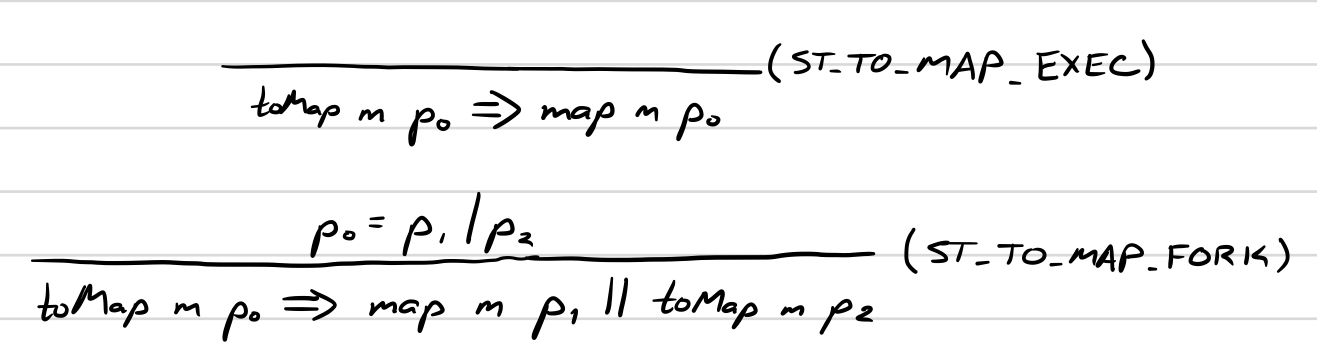
\includegraphics[scale=0.25]{img/ST_TO_MAP.jpeg}
%    \caption{Nondeterminism of two MapReduce reduction rules should enable
%             semantics to model any number of map task partitions, where each
%             task may be given \emph{any} partition of the data.}
%  \end{figure}
%\end{frame}
